\documentclass[a4paper, 11pt]{article}
\usepackage{comment} % enables the use of multi-line comments (\ifx \fi) 
\usepackage{lipsum} %This package just generates Lorem Ipsum filler text. 
\usepackage{fullpage} % changes the margin
\usepackage{graphicx}
\usepackage{color}
\usepackage{caption}
\usepackage{subcaption}
\graphicspath{ {./images/} }

\begin{document}
%Header-Make sure you update this information!!!!

\noindent
\large\textbf{Tema de cas\u{a}} \hfill \textbf{Programarea Aplica\c{t}iilor \^{i}n Timp Real} \\
\normalsize Echipa: B\u{a}lan Mihai, Ciobanu \c{S}tefan, Sp\^{i}nu Andrei  \hfill Sem. 2, 2021-2022 \\ 
\normalsize e-mail: mihai.balan1409@stud.acs.upb.ro,\\ stefan.ciobanu@stud.acs.upb.ro,\\ andrei.spinu1703@stud.acs.upb.ro  \\
\\
\large\textbf{\textcolor{blue}{Tem\u{a} de cas\u{a} PATR}}


\section{Introducere. Definire problem\u{a}}

\^{I}n acest\u{a} sec\c{t}iune va descris\u{a} problema care va fi implementat\u{a}.

\begin{itemize}
\item Problema bărbierului constă în existența unei frizerii și a unui bărbier, un scaun de frizerie și N scaune  de așteptare.
Dacă nu există clienți, frizerul se va odihni, însă dacă un client v-a apărea frizerul se va trezi si îl va tunde. Dacă toate scaunele de așteptare sunt ocupate, urmatorii clienți nu vor mai rămane în frizerie.
\end{itemize}

\section{Analiza problemei}

Aceast\u{a} sec\c{t}iune va cuprinde analiza cerin\c{t}elor.

Pentru realizarea acestei cerințe vom utiliza 3 taskuri:

\begin{itemize}
\item task-ul Barber.
\item task-ul Clienti.
\item task-ul Coada.
\end{itemize}


Mod de funcționare:
Bărbierul ajunge la salon și începe programul de lucru. Acesta așteaptă, stă și doarme, până când vine un client. Atunci când este adăugat clientul în coadă, se blochează MutexClient. După ce se adăugarea în coadă a fost finalizată, se deblochează MutexClient și se verifică disponibilitatea bărbierului, iar dacă acesta este liber, se blochează MutexBarber. Când bărbierul termină de tuns clientul, MutexBarber se deblochează. În cazul în care sala de așteptare este plină, clientul pleacă și se deblochează MutexClient. Taskul Coada calculează poziția de inserare pentru noul client. Dacă programul de lucru al bărbierului s-a terminat, nu mai sunt acceptați clienți în salon, urmând ca acesta să se închidă după ce bărbierul termină de tuns toți clienții deja existenți în sală.

\section{Definirea structurii aplica\c{t}iei}

\^{I}n aceast\u{a} sec\c{t}iune se vor identifica taskurile care compun aplica\c{t}ia, \^{i}n a\c{s}a fel \^{i}nc\^{a}t s\u{a} se foloseasc\u{a} toate conceptele prezentare la curs: 

\begin{itemize}
\item \textcolor{blue}{sincronizare}
\item \textcolor{blue}{excludere mutual\u{a}}
\item \textcolor{blue}{planificarea taskurilor pe condi\c{t}ie de timp}
\end{itemize}

Sincronizarea se va realiza folosind taskul Coada:
\begin{itemize}
\item TaskCoada - ține evidența numărului de persoane din camera de așteptare.
\end{itemize}

Excluderea mutuală:
\begin{itemize}
\item MutexBarber   - folosit pentru a exclude cazurile în care doi, sau mai mulți, clienți se așează simultan pe scaunul bărbierului. 
\item MutexClient   - folosit pentru a exclude cazurile în care doi, sau mai mulți, clienți intra simultan în frizerie. 
\end{itemize}

Planificarea taskurilor pe condi\c{t}ie de timp:
\begin{itemize}
\item Planificarea temporală se poate folosi pentru a realiza un program al frizerului, întrucât acesta nu lucrează 24/7, trebuie să știe și când să plece acasă.
\item O altă utilizarea a planificării temporale o reprezintă timpul pe care îl așteaptă clienții în camera de așteptare, până când să se hotărască să părăsească frizeria.
\end{itemize}



\section{Definirea solu\c{t}iei \^{i}n vederea implement\u{a}rii}

\^{I}n aceast\u{a} secțiune se va specifica modul \^{i}n care se va implementa aplica\c{t}ia:
\begin{itemize}
\item Linux Debian Xenomai, API C/POSIX
\item Arduino \c{s}i FreeRTOS
\end{itemize}

\paragraph{Se vor specifica mecanismele de sincronizare, comunicare \^{i}ntre taskuri \c{s}i de planificare a taskurilor pe condi\c{t}ie de timp pe care le-a\c{t}i ales din fiecare framework de progranare real-time.} De exemplu - explic\u{a}m detalii de implementare \^{i}n func\c{t}ie de limbaj:: 

\begin{itemize}
\item \^{i}n Java – nu exist\u{a} semafoare \^{i}n limbaj, trebuie definite software
\item \^{i}n C / Linux Debian Xenomai – exist\u{a} semafoare generalizate \c{s}i mutex-uri (corespunz\u{a}tor semafoarelor binare pentru sincronizarea firelor de execu\c{t}ie) 
\item \^{i}n FreeRTOS avem semafoare binare \c{s}i semafoare generalizate, precum si mutex-uri. 
\end{itemize}
\paragraph{}

\subsection*{Solu\c{t}ie de implementare}
\paragraph{}

Aleg mecanismele de sincronizare \c{s}i comunicare \^{i}ntre taskuri, prezent\^{a}nd organigramele taskurilor (e.g. \^{i}n Fig.~\ref{fig:taskuri}).

\begin{itemize}
\item aleg 2 mutex-uri, MutexBarber si MutexClient, cu val. ini\c{t}iale unlock
\end{itemize}
\paragraph{}
\paragraph{}

\begin{figure} [!htb]
\centering
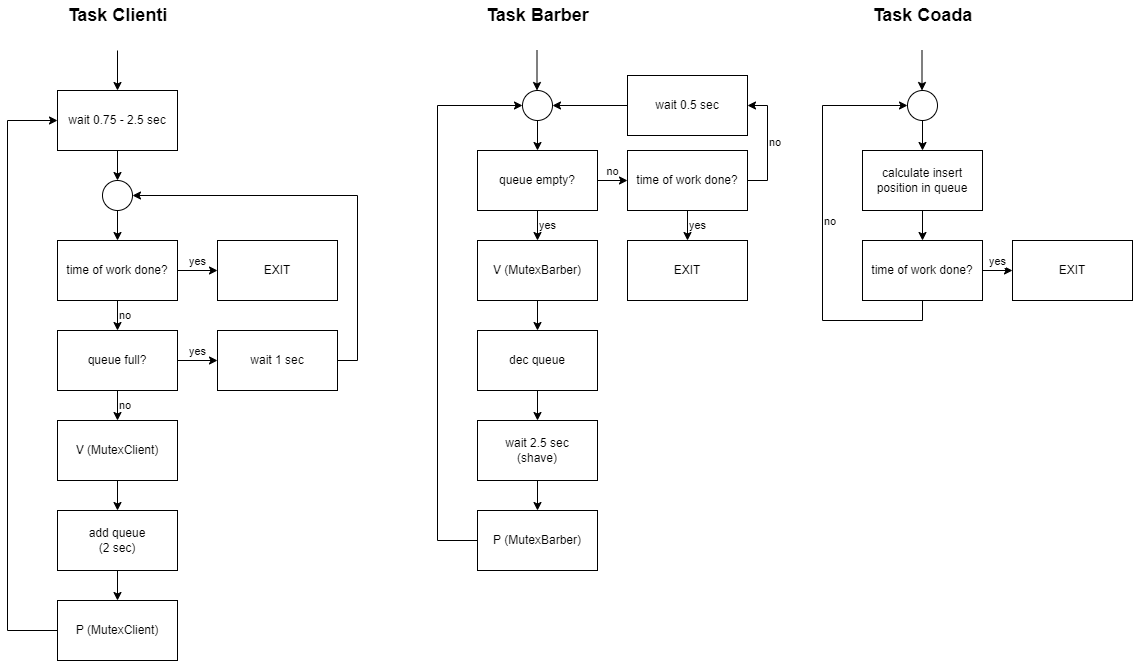
\includegraphics[width=17.5cm]{./images/Organigrama.png}
\caption{\label{fig:taskuri}Solu\c{t}ie implementare - organigrame taskuri}
\end{figure} 



\section{Implementarea solu\c{t}iei}

\^{I}n aceast\u{a} sec\c{t}iune se va prezenta codul aplica\c{t}iei. 

\paragraph{Se va comenta codul pentru a explica modul de lucru.}

\subsection*{Codul aplica\c{t}iei \^{i}n document}

\medskip
\medskip

\noindent
{\it \textbf{Task Barber}:}
{\small
\begin{verbatim}
    while(1) {
    if(scaune[0] and xSemaphoreTake(MutexBarber, portMAX_DELAY) == pdTRUE) {
      //Extragere din coada
      for(int i = 0; i < 7; i++) {
        scaune[i] = scaune[i + 1];
      }
      scaune[7] = 0;
      vTaskDelay(200 / portTICK_PERIOD_MS);
      digitalWrite(2, HIGH);
      Serial.println("Barbierul tunde o persoana.");
      //Barbierul tunde 2.5 secunde
      vTaskDelay(2500 / portTICK_PERIOD_MS);
      digitalWrite(2, LOW);
      Serial.println("Barbierul a tuns o persoana.");
      xSemaphoreGive(MutexBarber);
    }
    else if(!scaune[0]){
      //Oprire task
      if(!tunde) {
        Serial.println("Salonul s-a inchis, o zi buna!");
        vTaskDelete(NULL);
      }
      Serial.println("Nu e nimeni in coada!");
      vTaskDelay(500 / portTICK_PERIOD_MS);
    }
  }
\end{verbatim}

Se verifică dacă este vreun client în coadă și dacă bărbierul nu tunde pe altcineva, caz în care se blochează MutexBarber. Se realizează extragerea unui client din coadă și se așteaptă 200 de milisecunde până când acesta se așează pe scaunul bărbierului. După 2.5 secunde, bărbierul termină de tuns persoana  și se deblochează MutexBarber. În cazul în care coada este goală, bărbierul așteaptă clienți, iar dacă programul s-a terminat, taskul este oprit.
\paragraph{}

{\large\it \textbf{Task Clienti}:}
{\small
\begin{verbatim}
   while(1) {
    vTaskDelay(200 / portTICK_PERIOD_MS);
    //Calculare timp ramas pentru a mai primii clienti
    timpClienti = millis();
    if(timpClienti >= 60000) {
      tunde = false;
      Serial.println("Salonul se inchide, nu mai primim clienti!");
      vTaskDelete(NULL);
    }

    //Alegere aleatoare intre 2 clienti in intervalul 0.75 si 2.5 secunde 
    if(clientOk) {
      clientOk = false;
      timpRandom = random(750, 2500);
    }
    
    unsigned long timp = millis();
    if(timp - timpClient >= timpRandom) {
      //Mesaj pentru ca nu se poate adauga in coada un client
      if(pozitieInserare == -1) {
        Serial.println("Coada este plina!");
        digitalWrite(11, HIGH);
        vTaskDelay(1000 / portTICK_PERIOD_MS);
        digitalWrite(11, LOW);
        timpClient = timp;
        clientOk = true;
      }
      else if(pozitieInserare != -1 and xSemaphoreTake(MutexClient, portMAX_DELAY) == pdTRUE){
        //Ocupare scaun un salon de catre client, 1 secunda
        digitalWrite(12, HIGH);
        vTaskDelay(1000 / portTICK_PERIOD_MS);
        digitalWrite(12, LOW);
        scaune[pozitieInserare] = 1;
        Serial.println("A intrat o noua persoana!");
        timpClient = timp;
        clientOk = true;
        xSemaphoreGive(MutexClient);
      }
    }
  }
\end{verbatim}

Se verifică dacă s-a terminat programul de lucru al bărbierului, caz în care salonul nu mai primeste clienți, iar bărbierul v-a tunde doar persoanele care sunt în coadă. Se alege aleator, între 750 și 2500 de milisecunde, timpul de intrare al următorului client în salon. Acesta este adăugat în coadă dacă mai este loc liber, altfel o să plece. Timpul în care se face verificarea disponibilității durează o secundă. Dacă mai este loc liber pentru client în coadă, se blochează MutexClient, iar după ce acesta este adăugat, MutexClient este deblocat.
\paragraph{}

{\large\it \textbf{Task Coada}:}
{\small
\begin{verbatim}
   while(1) {
    //Calculare pozitie inserare
    int i;
    for(i = 0; i < 8; i++) {
      if(!scaune[i]) {
         break;
      }
    }
    if(i != 8) {
      pozitieInserare = i; 
    }
    else {
      pozitieInserare = -1;
    }     

    //Setare leduri
    for(int j = 0; j < 8; j++) {
      if(scaune[j]) {
        digitalWrite(j + 3, HIGH);   
      }
      else {
        digitalWrite(j + 3, LOW); 
      }
    }

    //Oprite task
    if(pozitieInserare == 0 and !tunde and xSemaphoreTake(MutexBarber, portMAX_DELAY) == pdTRUE) {
      vTaskDelete(NULL);
    }
  }
\end{verbatim}

Se calculează care este următorul scaun liber pe care poate să se așeze clientul nou venit. În cazul în care coada este liberă, programul salonului este terminat și bărbierul nu mai tunde pe nimeni, se poate bloca MutexBarber, taskul se oprește.
\paragraph{}\paragraph{}\paragraph{}

}



\section{Testarea aplica\c{t}iei si validarea solu\c{t}iei propuse}

Aceast\u{a} sec\c{t}iune include comentarii despre modul \^{i}n care se execut\u{a} programul. Se ob\c{t}ine ceea ce s-a specificat la pasul 1, \^{i}n cerin\c{t}e?

Programul rulează conform descrierii din cadrul pasului 1, astfel obținându-se gestionarea și sincronizarea task-urilor pentru îndeplinirea cerinței.

\paragraph{}

\begin{figure} [!htb]
\centering
\begin{subfigure}{.5\textwidth}
  \centering
  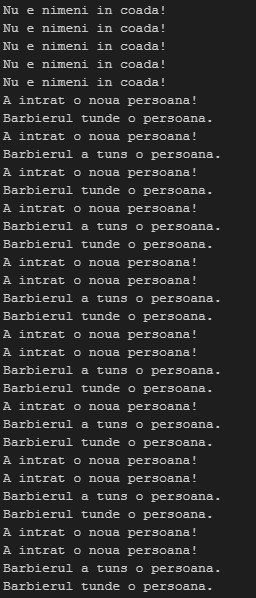
\includegraphics[width=5cm]{./images/Rezultat1.jpeg}
  \caption{}
  \label{fig:sub1}
\end{subfigure}%
\begin{subfigure}{.5\textwidth}
  \centering
  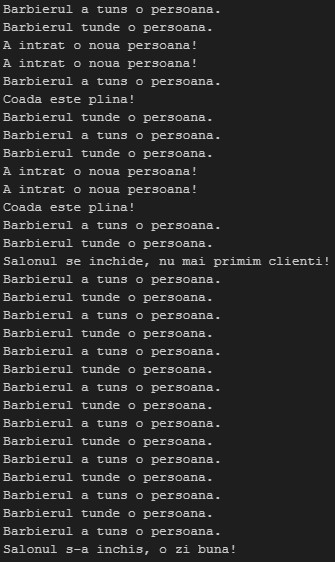
\includegraphics[width=6.95cm]{./images/Rezultat2.jpeg}
  \caption{}
  \label{fig:sub2}
\end{subfigure}
\caption{Rezultat execuție aplicație - 8 locuri în coadă}
\label{fig:taskuri}
\end{figure}

\begin{figure} [!htb]
\centering
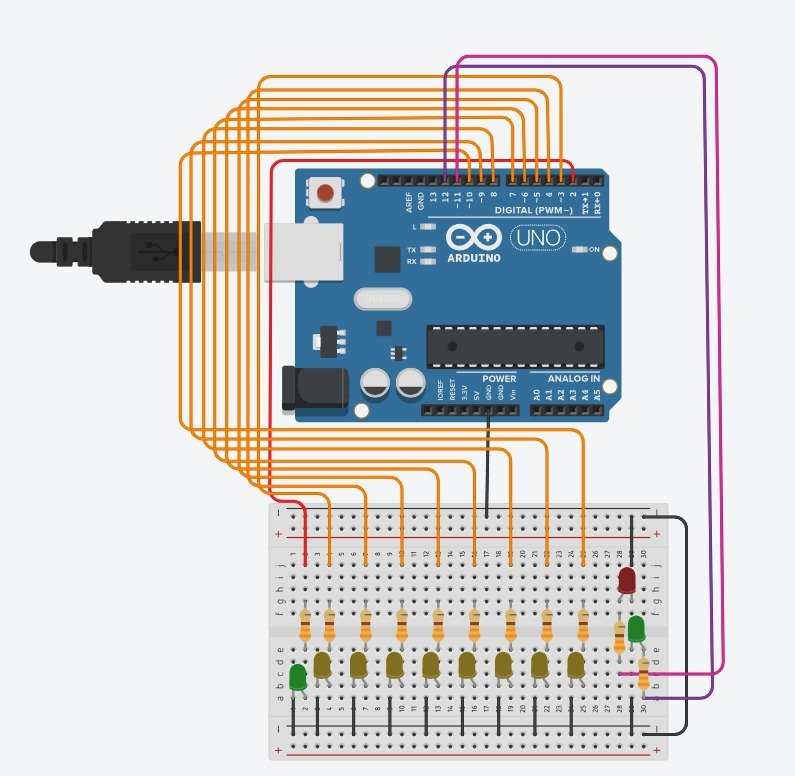
\includegraphics[width=12cm]{./images/Simulink.jpeg}
\caption{\label{fig:taskuri}Implementare Simulink}
\end{figure}

\end{document}
